% 模板出处:https://zhuanlan.zhihu.com/p/379360037

\documentclass[12pt, a4paper, oneside]{book}
\usepackage{ctex}
\usepackage{amsmath, amsthm, amssymb, bm, graphicx, hyperref, mathrsfs, enumitem}
\hypersetup{
    colorlinks=true,
    linkcolor=blue,
    filecolor=blue,      
    urlcolor=blue,
    citecolor=cyan,
}
\usepackage{pgfplots}
\pgfplotsset{compat=newest}
\usepackage{comment}
\usepackage{titlesec,titleps} % 添加 titlesec 宏包
\titleclass{\section}{straight} % 清除默认章节格式

% 章节格式统一设置
\titleformat{\section}[runin]
  {\normalfont\bfseries}
  {\thesection.}
  {-0.5em}
  {\quad}
  
\titleformat{\subsection}[runin]
  {\normalfont\bfseries}
  {\thesubsection.}
  {-0.3em}
  {\quad}

% 间距微调
\titlespacing*{\section}
  {0pt}
  {1.2ex plus 0.5ex minus 0.2ex}
  {0.3em}

\titlespacing*{\subsection}
  {15pt} % 二级标题增加缩进
  {0.8ex plus 0.3ex minus 0.1ex}
  {0.2em}

\renewcommand{\thesection}{\arabic{section}}
\renewcommand{\thesubsection}{\arabic{section}\arabic{subsection}}

% 图编号格式调整
\numberwithin{figure}{section}

% 定理环境样式调整
\theoremstyle{definition}
\newtheorem{theorem}{定理}[section]
\newtheorem{lemma}[theorem]{引理}
\newtheorem{definition}[theorem]{定义}
\newtheorem{example}[theorem]{例}
\newtheorem{proposition}[theorem]{命题}

% 页眉页脚设置(来自于 titleps 宏包)
% 设置页眉为楷体
\newpagestyle{main}{
    \sethead{\kaishu \sectiontitle}{}{\kaishu \thepage}
}
\pagestyle{main}

\title{{\Huge{\textbf{测度与概率 Notes}}}}
\author{Liu Fuzhou}
\date{\today}
\linespread{1.5}






\begin{document}

\maketitle

\pagenumbering{roman}
\setcounter{page}{1}

%\begin{comment}
\begin{center}
    \Huge\textbf{前言}
\end{center}~\

要看偏微分方程,就要先看泛函分析. 要看泛函分析,就要先看实分析. 泛函分析和实分析对随机分析也是重要的. 无论如何也绕不开 $L^p$ 空间. 可见掌握实分析十分重要. 以前其实也看过这个主题的书,结果后来都忘了. 看来做一些有形的笔记是很有必要的. 不需要特别详细,提纲挈领即可.

主要参考文献:
\begin{enumerate}
\item[1.] 近代概率引论:测度、鞅和随机微分方程. 袁震东. 科学出版社, 1991.
\item[2.] 测度与概率教程. 任佳刚,巫静. 科学出版社, 2018.
\item[3.] Measure, Integration \& Real Analysis. Sheldon Axler. Springer, 2020.
\end{enumerate}

~\\
\begin{flushright}
    \begin{tabular}{c}
        Liu Fuzhou\\
        \today
    \end{tabular}
\end{flushright}
%\end{comment}

\newpage
\pagenumbering{Roman}
\setcounter{page}{1}
\tableofcontents
\newpage
% 生成图表目录
\listoffigures
\newpage
\setcounter{page}{1}
\pagenumbering{arabic}


\section{集列的极限}
首先比较重要的概念就是集列的上极限与下极限. 集列 $\{A_n\}_{n\in\mathbb N}$ 的上极限就是落到其中无限多个集合的元素所做成的集合,也即 $\limsup_{n\to\infty}A_n=\bigcap_{n=1}^\infty\bigcup_{k=n}^\infty A_k.$ 
下极限就是除去有限多个集合后,落到所有集中的元素所做成的集合,也即 $\liminf_{n\to\infty}A_n=\bigcup_{n=1}^\infty\bigcap_{k=n}^\infty A_k.$ 换言之也即“最终落到集列” $A_n$ 中的那些元素之全体.
显然,下限集中的元素也都落到上限集之中,也即 $\liminf A_n\subset \limsup A_n.$ 如果集列 $A_n$ 的上限集与下限集相等,那么就说集列 $A_n$ 收敛,并称 $A=\liminf A_n=\limsup A_n$ 为集列 $A_n$ 的极限. 这个极限是关于集合包含的偏序关系说的. 
与实数的情况类似,有单调集列的收敛定理:如果 $A_n\uparrow$ 是单调递增的,那么 $\lim A_n=\bigcup_n A_n.$ 类似地,如果 $A_n\downarrow$ 是单调递减的,那么 $\lim A_n=\bigcap_n A_n.$ 


\begin{example}
    设 $\{A_n\}_{n\in\mathbb N}$ 为单调减少集列. 证明 
    \begin{equation*}
        A_1=\sum_{n=1}^\infty (A_n-A_{n+1}) + \bigcap_{n=1}^\infty A_n
    \end{equation*}
\end{example}
\begin{proof}
首先,右边的每个集合都含于 $A_1.$ 因此右边含于 $A_1.$ 其次,若 $x\in A_1$ 且 $x\notin \bigcap_{n=1}^\infty A_n$, 则 $x\in \sum_{n=1}^\infty (A_n-A_{n-1})$ 且 $x\notin \bigcap_{n=1}^\infty A_n.$ 因此 $A_1$ 也是单调递减的. 最后,若 $x\in \bigcap_{n=1}^\infty A_n$, 则存在某个 $n>1,$ 使得 $x\notin A_n.$ 令 $n_0$ 为最小的这种 $n,$ 那么就有 $x\notin A_{n_0},\ x\in A_{n_0-1}.$ 于是就有 $x\in \sum_{n=1}^\infty (A_n-A_{n-1}).$ 这就证明了 
$A_1\subset \sum_{n=1}^\infty (A_n-A_{n+1}) + \bigcap_{n=1}^\infty A_n.$ 
\end{proof}

\section{Riemann 积分} 
还是用 \cite{Axler_2020} 作为参考书比较好,还是彩色的. 我还是比较喜欢 Riemann 积分的,最开始是在梅加强的书上学的. 比较重要的技术就是证明 Darboux 上和总是大于等于 Darboux 下和那里,需要用到两个 partition 的 merge. 也就是说,用到了有界闭区间的 partition 全体构成一个 directed set 的性质. Darboux 上和与 Darboux 下和之差就是所谓的函数振幅 
$\Omega_\mathcal P (f)=\sum_{i} (\sup_{x_{i-1}\leq x\leq x_i} f-\inf_{x_{i-1}\leq x\leq x_i})(x_i-x_{i-1}),$ 这里 $\mathcal P=\{a=x_0<x_1<\cdots<x_n=b\}$ 是所讨论的具体的分割. 

如果向 partition 的点集增加元素,也即使得分割变得更细,那么结果就是上和不增,下和不减. 这就导致了两个极限 $\lim_{\mathcal P} \mathcal L(f,\mathcal P,[a,b])$ 和 $\lim_{\mathcal P} \mathcal U(f,\mathcal P,[a,b]),$ 称为 Riemann 下积分 $\underline{\int}$ 和上积分 $\overline{\int}$. 这两个极限是关于 partition 全体所具有的 directed set 结构说的, 也就是说是 net 的极限. 由于下和不大于上和,也即 $\mathcal L\leq \mathcal U,$ 因此这两个极限之间也有关系
\begin{equation}
    \underline{\int}_a^b f(x)\ \mathrm dx\leq  \overline{\int}_a^b f(x)\ \mathrm dx
\end{equation}
如果 Riemann 上下积分相等,就说 $f$ 在 $[a,b]$ 上 Riemann 可积,其积分 $\int_a^b f(x)\ \mathrm dx$ 就定义为上下积分的共同值. 

任意分割 $\mathcal P$ 都将区间 $[a,b]$ 分成 $\#(\mathcal P)-1$ 个首尾相接的闭区间 $[x_0,x_1],\cdots,[x_{n-1},x_n].$ 从每个闭区间挑选一个元素出来,就可以做成一个集合 $\Delta.$ 这种挑选当然是不唯一的. 称这种通过在每个闭区间中挑出一个元素所形成的集合为与 partition $\mathcal P$ 相伴的一个点集. 
设 $\{\mathcal P_n\}_{n\in\mathbb N}$ 是任意一列 partition, 并且 $\{\Delta_n\}_{n\in\mathbb N}$ 是一列与之相伴的点集,每个 $\Delta_n$ 中元素形如 $\Delta_n=\{\xi_1,\cdots,\xi_{\#(\mathcal P_n)-1}\},$ 那么就可以考虑 Riemann 和所形成的数列
\begin{equation}
    \mathcal R_n:=\mathcal R(f,\mathcal P_n,\Delta_n,[a,b])=\sum_{i=1}^{\#(\mathcal P_n)-1} f(\xi_i)(x_{i}-x_{i-1})
\end{equation}
显然有 $\mathcal L(f,\mathcal P_n,[a,b])\leq \mathcal R_n\leq \mathcal U(f,\mathcal P_n,[a,b]).$ 因此有
\begin{equation}\label{eq:Riemann limit inequalities}
    \underline{\int}_a^b f(x)\ \mathrm dx\leq \liminf \mathcal R_n\leq \limsup \mathcal R_n\leq  \overline{\int}_a^b f(x)\ \mathrm dx
\end{equation}

这就表明,如果 $\mathcal R_n$ 有收敛子列的话,那么该子列的极限就必定位于上下积分之间.  当然了,如果 $f$ 是 Riemann 可积的,这个极限就必定等于 $\int_a^b f(x)\ \mathrm dx.$ 


以上讨论了利用 partition 的全体所组成的集合之上的 directed set 结构来定义的 Riemann 积分. 下面考虑利用 Riemann 和关于 partition 的 mesh 的极限的途径. 这就是说,把 Riemann 积分定义为极限
\begin{equation}\label{eq:Riemann_limit}
    \lim_{\|\mathcal P\|\to 0} \mathcal R(f,\mathcal P,\Delta,[a,b])
\end{equation}
其中 $\|\mathcal P\|=\max_{i}|x_{i}-x_{i-1}|$ 是 partition 的 mesh. 这个极限其实相当强,因为其定义只涉及 partition, 对相伴的点集 $\Delta$ 没什么要求.  

由不等式 \eqref{eq:Riemann limit inequalities} 可知,如果两种定义下的 Riemann 积分均存在,那么它们的值必定相等. 因此,两种定义的等价性的证明就归结于证明其存在性的等价性.


要证明两种定义的等价性,首先要注意到,上下积分之差恰好等于函数振幅的下确界 $\inf_{\mathcal P}\Omega_\mathcal P(f).$ 这就是说 $\lim_{\mathcal P} (\mathcal U(f,\mathcal P,[a,b])-\mathcal L(f,\mathcal P,[a,b]))=\inf_{\mathcal P}\Omega_\mathcal P(f),$ 或者说 $\lim_{\mathcal P}\Omega_\mathcal P(f)=\inf_{\mathcal P}\Omega_\mathcal P(f).$ 
事实上,设 $\varepsilon>0,$ 那么由 net 的极限的定义,存在 partition $\mathcal P_0,$ 使得任意细于 $\mathcal P_0$ 的分割 $\mathcal P$ 都满足 $|\Omega_{\mathcal P_0}(f)-\lim_{\mathcal P} \Omega_{\mathcal P}(f)|<\varepsilon.$ 
另一方面,由下确界的定义,存在 partition $\mathcal P_1$ 使得 $\Omega_{\mathcal P_1}(f)< \inf_{\mathcal P}\Omega_{\mathcal P}(f)+\varepsilon.$
取分割 $\mathcal P_2$ 为 $\mathcal P_0$ 与 $\mathcal P_1$ 的 merge, 那么就有 
\begin{equation}
    \lim_{\mathcal P}\Omega_{\mathcal P}(f)-\varepsilon< \Omega_{\mathcal P_2}(f)\leq \Omega_{\mathcal P_1}(f)<\inf_{\mathcal P}\Omega_{\mathcal P}(f)+\varepsilon
\end{equation}
于是 $\inf_{\mathcal P}\Omega_{\mathcal P}(f)\leq \lim_{\mathcal P}\Omega_{\mathcal P}(f)<\inf_{\mathcal P}\Omega_{\mathcal P}(f)+2\varepsilon.$ 这就证明了 
\begin{equation}
    \overline{\int}_a^b f(x)\ \mathrm dx - \underline{\int}_a^b f(x)\ \mathrm dx = \inf_{\mathcal P}\Omega_{\mathcal P}(f)
\end{equation}

假如极限 \eqref{eq:Riemann_limit} 存在,其值记为 $A,$ 那么对于任意的 $\varepsilon>0,$ 存在 $\delta>0,$ 使得只要 partition 的 mesh 小于 $\delta,$ 就有 $|\mathcal R(f,\mathcal P,\Delta,[a,b])-A|<\varepsilon.$ 
现在固定分割 $\mathcal P,$ 那么由于该不等式对于任意与 $\mathcal P$ 相伴的点集 $\Delta$ 都成立,因此有 $\Omega_{\mathcal P}(f)\leq 2\varepsilon.$ 这就证明了 $\inf_{\mathcal P}\Omega_{\mathcal P}(f)=0,$ 因而上下积分相等. 

反之,要从上下积分相等导出极限 \eqref{eq:Riemann_limit} 的存在性,还需要证明一个基于 partition 的 mesh 估计的技术性引理:
\begin{lemma}\label{lemma:mesh estimate}
    设 $\mathcal P,\mathcal P'$ 为区间 $[a,b]$ 的两个 partition, $M=\sup_{x\in [a,b]}|f(x)|,$ 那么就有不等式 
    \begin{equation}\label{eq:mesh estimate}
        \Omega_{\mathcal P}(f) \leq \Omega_{\mathcal P'}(f) + (\#(\mathcal P')-2)M\|\mathcal P\|
    \end{equation}
\end{lemma}

事实上,如果向 $\mathcal P$ 中添加一个新元素 $y,$ 譬如说插入到区间 $[x_k,x_{k+1}]$ 中,那么所形成的新分割 $\mathcal P''$ 的 Darboux 和与 $\mathcal P$ 的 Darboux 的差异仅来自于区间 $[x_k,x_{k+1}]$ 的贡献,也即
\begin{equation}
    \Omega_{\mathcal P''}(f)-\Omega_{\mathcal P}(f)=\omega_{x_k\leq x\leq y}f(x) (y-x_k)+ \omega_{y\leq x\leq x_{k+1}}f(x) (x_{k+1}-y) - \omega_{x_k\leq x\leq x_{k+1}}f(x) (x_{k+1}-x_k)
\end{equation}
考虑到 $\omega_{x_k\leq x\leq y}-\omega_{x_k\leq x\leq x_{k+1}}$ 和 $\omega_{y\leq x\leq x_{k+1}}-\omega_{x_k\leq x\leq x_{k+1}}$ 都落到区间 $[-M,M]$ 内,因此 $\Omega_{\mathcal P''}(f)-\Omega_{\mathcal P}(f)$ 的绝对值被 $M(x_{k+1}-x_k)$ 控制, 
从而也被 $M\|\mathcal P\|$ 控制. 这就导出了 $|\Omega_{\mathcal P''}(f)-\Omega_{\mathcal P}(f)|\leq M\|\mathcal P\|.$ 类似地,如果向 $\mathcal P''$ 中再插入一个新元素得到新分割 $\mathcal P''',$那么同样有
\begin{equation}
    |\Omega_{\mathcal P'''}(f)-\Omega_{\mathcal P''}(f)|\leq M\|\mathcal P''\|
\end{equation}
由于 $\mathcal P'''$ 细于 $\mathcal P,$ 因此 $\|\mathcal P'''\|\leq \|\mathcal P\|.$ 因此 $\Omega_{\mathcal P'''}(f)-\Omega_{\mathcal P''}(f)$ 的绝对值也被 $M\|\mathcal P\|$ 控制,从而有 $|\Omega_{\mathcal P'''}(f)-\Omega_{\mathcal P}(f)|\leq 2 M\|\mathcal P\|.$ 
现在考虑 $\mathcal P$ 与 $\mathcal P'$ 的 merge $\mathcal S,$ 其可以通过反复向 $\mathcal P$ 中插入元素来得到,插入次数至多为 $ \#(\mathcal P')-2$ 次. 因此就有
\begin{equation}
    \Omega_{\mathcal P}(f)-(\#(\mathcal P')-2)M\|\mathcal P\|\leq \Omega_{\mathcal S}(f)\leq \Omega_{\mathcal P'}(f)
\end{equation}
这就导出了不等式 \eqref{eq:mesh estimate}. 这个引理最初是在 \cite{Mei_2011} pp.213 看到的.

作为引理 \ref{lemma:mesh estimate} 的一个推论,立刻可以导出
\begin{equation}\label{eq:Riemann_limit_mesh_inf}
    \lim_{\|\mathcal P\|\to 0} \Omega_{\mathcal P}(f)=\inf_{\mathcal P}\Omega_{\mathcal P}(f)
\end{equation}
这是因为,设 $\varepsilon>0,$ 那么由下确界的定义可知存在 partition $\mathcal P_0,$ 使得 $\Omega_{\mathcal P_0}(f)<\inf_{\mathcal P}\Omega_{\mathcal P}(f)+\varepsilon.$ 
记 $N=\#(\mathcal P_0)-2,$ 那么当 partition 的 mesh 小于 $\varepsilon/(MN)$ 时,由引理 \ref{lemma:mesh estimate} 可知
\begin{equation}
    \Omega_{\mathcal P}(f)\leq\Omega_{\mathcal P_0}(f)+(\#(\mathcal P')-2)M\|\mathcal P\|<\inf_{\mathcal P}\Omega_{\mathcal P}(f)+2\varepsilon
\end{equation}
这就证明了 \eqref{eq:Riemann_limit_mesh_inf} 式. 类似地可以证明
\begin{equation}\label{eq:Riemann_limit_mesh_upper_lower}
    \lim_{\|\mathcal P\|\to 0} \mathcal L(f,\mathcal P,[a,b])=\underline{\int}_a^b f(x)\ \mathrm dx,\ \lim_{\|\mathcal P\|\to 0} \mathcal U(f,\mathcal P,[a,b])=\overline{\int}_a^b f(x)\ \mathrm dx.
\end{equation}

现在假设 Riemann 上下积分相等,也即 $\lim_{\|\mathcal P\|\to 0}\Omega_{\mathcal P}(f)=0,$ 那么对于任意的 $\varepsilon>0,$ 存在 $\delta>0,$  使得只要 partition 的 mesh 小于 $\delta,$ 就有
$|\mathcal U-\overline{\int}|,|\mathcal L-\underline{\int}|< \varepsilon.$ 自然,此时由不等式 \eqref{eq:Riemann_limit_mesh_upper_lower} 可知
\begin{equation}
    \underline{\int}_a^b f(x)\ \mathrm dx-\varepsilon<\mathcal L(f,\mathcal P,[a,b])\leq \mathcal R(f,\mathcal P,\Delta,[a,b])\leq \mathcal U(f,\mathcal P,[a,b])\leq \overline{\int}_a^b f(x)\ \mathrm dx+\varepsilon
\end{equation}
这就证明了极限 \eqref{eq:Riemann_limit} 的存在性.

容易验证闭区间上的连续函数是 Riemann 可积的. 这主要用到了其一致连续性.

\section{Riemann 积分的若干缺陷}

Riemann 积分的一些缺陷:
\begin{enumerate}
    \item 如果函数的连续性较差,则其 Riemann 可积性也较差:典型的例子就是 Dirichlet 函数.
    \item 无界函数的 Riemann 可积性较差(反常积分):一个例子就是取一列可求出瑕积分的函数 $f_k(x),$ 使得每个函数的瑕点恰好对应区间 $[0,1]$ 上的一个有理数,最终导致无法通过划分区间的办法求出函数 $f:=\sum_k {f_k\over 2^k}$ 的瑕积分. 这里其实是说,
          如果将面积的次可加性推广到可数的情况,那么通常的 Riemann 积分就不太够用了. 毕竟这样构造出的 $f$ 多多少少是个较为奇怪的函数,这种例子更偏向于理论意义. 
    \item Riemann 积分与极限的可交换性较差:这个问题看起来是最为致命的. 可以构造出一列函数 $f_k,$ 它们的 Riemann 积分均为零,但其逐点收敛到 Dirichlet 函数. 虽然可以证明,如果一致有界的可积函数列的逐点极限函数是 Riemann 可积的,那么其积分与极限可以交换位置,也即 $\lim_{n} \int_a^b f_n = \int_a^b \lim_n f_n,$ 但其证明 
          却非常复杂,并且也绕不过使用测度的思想. 这个缺陷使得 Riemann 积分在理论上使用起来尤为不便. 
\end{enumerate}

\begin{example}
    定义闭区间 $[0,1]$ 上的函数 $f$ 为
    \begin{equation}
        f(x)=\begin{cases}
            0, & \text{若 $x$ 为无理数}\\
            {1\over n}, & \text{若 $x$ 为有理数,且 $n$ 为形如 $x={m\over n}$ 的表达式中的最小正整数 $n$}
        \end{cases}
    \end{equation}
    证明 $f$ 是 Riemann 可积的,并计算其积分值.
\end{example}
显然 $f$ 的每一个 Darboux 下和都为零,因此 $\underline{\int}_0^1 f = 0.$ 下面证明 $f$ Riemann 可积. 只需构造出一列 partition $\mathcal P_n,$ 使得 $\lim_n \Omega_{\mathcal P_n}(f)=0$ 即可. 由于 $\mathcal L\equiv 0,$ 因此只需证明 $\lim_n \mathcal U(f,\mathcal P_n,[0,1])=0.$
事实上,对于任意的 $n,$ 满足 $f(x)=1/n$ 的 $[0,1]$ 内的有理数至多有 $n+1$ 个,因此其数目有限. 自然,可以适当地划分区间,得到分割 $\mathcal P_n,$ 使得满足 $f(x)\geq 1/n,$ 也即 $f(x)=1,1/2,\cdots,1/n$ 的全体有理数 $x$ 所在的区间的总长不超过 $1/n.$ 自然,$f$ 在剩下的那些区间上的上确界均小于 $1/n.$ 于是就有
\begin{equation}
    \begin{aligned}
        \mathcal U(f,\mathcal P_n,[0,1])=&\sum_{\text{$f(x)\geq 1/n$ 的 $x$ 所在区间 $[x_{i-1},x_{i}]$}} \sup_{x_{i-1}\leq x\leq x_i}f(x)(x_i-x_{i-1})\\
        &+\sum_{\text{其余区间 $[x_{i-1},x_{i}]$}}\sup_{x_{i-1}\leq x\leq x_i}f(x)(x_i-x_{i-1})  \\
        <& {1\over n}-{1\over n}\left(1-{1\over n}\right) \\
        =&{2\over n}-{1\over n^2}
    \end{aligned}
\end{equation}
于是就有 $\lim_n \mathcal U(f,\mathcal P_n,[0,1])=0.$ 因此 $f$ 是 Riemann 可积的,并且其 Riemann 积分为 $\int_0^1 f=0.$


\begin{example}
    Riemann 积分与极限交换时,一致有界条件不可去掉.
\end{example}
事实上,构造单位区间 $[0,1]$ 上的连续函数列
\begin{equation}\label{eq:swap_limit_counterexample}
    f_n(x) = \begin{cases}
        n^2 x, & \text{若 $0\leq x\leq 1/n$}\\
        2n-n^2x, & \text{若 $1/n<x\leq 2/n$}\\
        0&\text{若 $x>2/n$}
    \end{cases}
\end{equation}

\begin{figure}[]
    \centering
    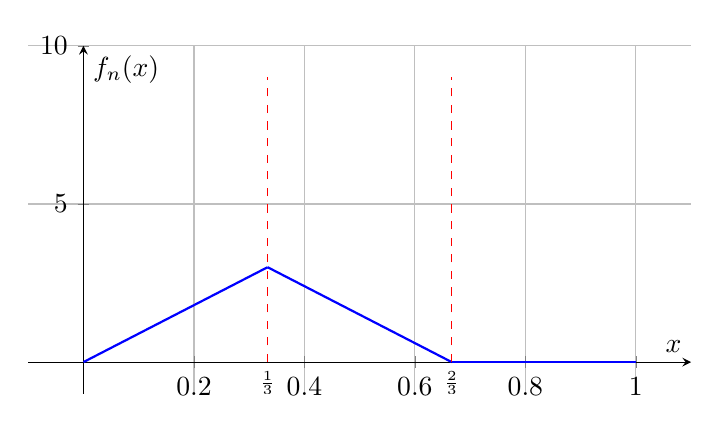
\begin{tikzpicture}
    \begin{axis}[
        axis lines = middle,
        xlabel = {$x$},
        ylabel = {$f_n(x)$},
        ymin = -1, ymax = 10,
        xmin = -0.1, xmax = 1.1,
        domain = 0:1,
        samples = 100,
        grid = major,
        width=10cm,
        height=6cm,
    ]
    
    % Define n
    \def\n{3}
    
    % Plot the function
    \addplot [thick, blue, domain=0:1/\n] {(\n)^2 * x};
    \addplot [thick, blue, domain=1/\n:2/\n] {2*\n - (\n)^2 * x};
    \addplot [thick, blue, domain=2/\n:1] {0};
    
    % Add vertical lines at x = 1/n and x = 2/n
    \draw [dashed, red] (axis cs:1/\n,0) -- (axis cs:1/\n,9);
    \draw [dashed, red] (axis cs:2/\n,0) -- (axis cs:2/\n,9);
    
    % Add labels for the vertical lines
    \node [below, font=\scriptsize] at (axis cs:1/\n,0) {$\frac{1}{3}$};
    \node [below, font=\scriptsize] at (axis cs:2/\n,0) {$\frac{2}{3}$};
    
    \end{axis}
    \end{tikzpicture}
    \caption{Graph of the piecewise function \( f_n(x) \) depicted by equation \eqref{eq:swap_limit_counterexample} for \( n=3 \).}
    \label{fig:fn}
\end{figure}

那么就有 $\int_0^1 f_n = 1,$ 以及 $\lim_n f_n(x)\equiv 0.$ 这是因为 $f_n(x)$ 也就只在开区间 $(0,2/n)$ 上不为零,该区间随着 $n\to\infty$ 而消失.
因此,极限函数 $f:=\lim_n f_n$ 是连续的,并且有 $\int_0^1 f=0.$ 因此
\begin{equation}
    \lim_n \int_0^1 f_n = 1\neq 0=\int_0^1 \lim_n f_n
\end{equation}
当然,$f_n$ 不是一致有界的:$\sup_{x\in [0,1]}f_n(x)=n,$ 因此 $f_n(x)$ 不可能被某个有限的数所一致控制.


\section{外测度} 外测度的概念是经典的:对 $\mathbb R$ 的任意子集 $A,$ 都可定义其外测度 $|A|$ 为覆盖 $A$ 的开区间列的总长度之下确界,也即 $|A|=\inf_{A\subset\bigcup_n I_n} \sum_n \ell(I_n).$
这总是定义良好的. 如果某个 $\ell(I_n)$ 为 $+\infty,$ 那么显然 $\sum_n \ell(I_n)=+\infty.$ 反之,$\sum_n \ell(I_n)$ 是一个非负项的数项级数. 
自然,非负项级数要么收敛,要么发散到 $+\infty.$ 因此,如果将 $+\infty$ 也作为一个合法的长度值,
那么 $\sum_n \ell(I_n)$ 总是有定义的,并且总是大于等于零. 因此任意的实数集 $A$ 的外测度总是有定义的.

\begin{example}
    可数集的外测度为零.
\end{example}
设 $A=\{a_n\}_{n\in\mathbb N},\ \varepsilon>0,$ 那么可以构作区间列 $I_n=(a_n-\varepsilon/2^n,a_n+\varepsilon/2^n),$ 使得 $A\subset \bigcup_n I_n,$ 于是 
\begin{equation}
    |A|\leq \sum_n \ell(I_n)=\sum_n {\varepsilon\over 2^{n-1}}=2\varepsilon
\end{equation}
这就证明了 $|A|=0.$ 

特别的,有理数集 $\mathbb Q$ 的外测度为零. 这表明外测度的性质至少要比 Jordan 测度要好,因为 $\mathbb Q\cap [0,1]$ 的 Jordan 测度正是 Dirichlet 函数的 Riemann 积分,因而是不存在的.

如果实数集 $A$ 含于 $B,$ 那么任意覆盖了 $B$ 的开区间列也覆盖了 $A,$ 因而 $|A|\leq |B|.$ 因此外测度与集合的包含关系的相容性良好. 此外,由于平移变换并不改变开区间的长度,并且将开区间变为开区间,并且还是可逆的,因此任意实数集 $A$ 平移 $t$ 距离后,其外测度保持不变:$|A+t|=|A|.$ 这就是说外测度具有平移不变性.

外测度最为重要的一条性质恐怕就是次可数可加性了.
\begin{theorem}
    外测度具有次可数可加性:$|\bigcup_n A_n|\leq \sum_n |A_n|.$
\end{theorem}
首先,如果某个集合 $A_n$ 的外测度为 $+\infty,$ 那么结论显然成立. 下面假设所有 $|A_n|$ 都是有限的. 设 $\varepsilon>0.$ 对于任意固定的 $n,$ 根据外测度的定理,可以找到一列开区间 $\{I_{n,k}\}_{k\in\mathbb N},$ 使得
\begin{equation}
    \sum_k \ell(I_{n,k})<|A_n|+{\varepsilon\over 2^n}
\end{equation}
自然,记所有这些区间 $I_{n,k}$ 所做成的集合为 $X,$ 那么映射 $\mathbb N\times\mathbb N\to X,\ (n,k)\mapsto I_{n,k}$ 可以重新排列顺序为 $\mathbb N\to X,\ j\mapsto I_{n(j),k(j)}.$ 这一列区间 $I'_j:=I_{n(j),k(j)}$ 覆盖了 $\bigcup_n A_n,$ 并且对于每个正整数 $p\in\mathbb N,$ 记 $n(1),\cdots,n(p)$ 中的最大值为 $N(p),$ 则有
\begin{equation}
    \sum_{j=1}^p \ell(J_j) \leq \sum_{n=1}^{N(j)} \sum_k \ell(I_{n,k}) \leq \sum_n\sum_k \ell(I_{n,k})<\sum_n |A_n|+\varepsilon
\end{equation}
于是 $\sum_j \ell(J_j)\leq\sum_n |A_n|+\varepsilon.$ 
这就证明了 
\begin{equation}\label{eq:outer_measure_subadditivity}
    \left|\bigcup_n A_n\right|\leq \sum_n |A_n|
\end{equation}
作为一个简单推论,外测度也具有次有限可加性:$|A_1\cup\cdots\cup A_n|\leq \sum_{i=1}^n |A_i|.$ 

下面来计算有界区间的外测度. 从几何上来看,开区间 $(a,b)$ 的外测度应该就等于其长度 $b-a.$ 严格的证明稍微麻烦一些,需要借助有界闭区间的紧性. 首先,$(a,b)$ 与 $[a,b]$ 的外测度相同:$|(a,b)|\leq |[a,b]|\leq b-a,$ 并且由 $[a,b]\subset (a-\varepsilon,b+\varepsilon),$ 以及 
$|(a-\varepsilon,b+\varepsilon)|\leq |(a,b)|+2\varepsilon$ 可得 $[a,b]\leq (a,b).$ 这就证明了开区间 $(a,b)$ 的外测度与其闭包相同. 另一方面,由 $[a,b]$ 的紧性可知,任意覆盖了 $[a,b]$ 的开区间列 $I_n$ 都存在有限子覆盖 $J_1,\cdots,J_p.$ 
下面只需证明 $\sum_{i=1}^p \ell(J_i)\geq b-a$ 即可. 最简单的证法是用归纳法(\cite{Axler_2020} pp. 20). 当 $p=1$ 时结论显然成立. 假设该结论对 $p\leq k$ 成立,那么当 $p=k+1$ 时,设 $[a,b]$ 被开区间 $J_1,\cdots,J_p$ 中的某个 $J_s=(c,d)$ 所覆盖,那么若 $c\leq a,$ 则 $\ell((c,d))\geq b-a,$ 故结论成立. 
若 $c>a,$ 则闭区间 $[a,c]$ 被 $k$ 个开区间 $\{J_i\}_{1\leq i\leq p,\ i\neq s}$ 所覆盖,于是由归纳假设即知 $\sum_{i\neq s}\ell(J_i)\geq c-a.$ 于是就有 $\sum_{i=1}^p \ell(J_i)\geq (c-a)+(b-c)=b-a,$ 因此总是有 
$\sum_n \ell(I_n)\geq b-a.$ 这就证明了 $|[a,b]|=b-a,$ 因而开区间 $(a,b)$ 的外测度也等于 $b-a.$

利用区间的外测度还可以给出区间的不可数性的另一个证明.
\begin{example}
    非空区间是不可数的.
\end{example}
事实上,由于可数集的外测度为零,而非空区间的外测度都大于零,因而非空区间不可能是可数集. 这就证明了结论.

\section{外测度的缺点:不可加性} Vitali 提供了集合的不交并的外测度不等于各自外测度之和的一个例子. 
\begin{example}\label{ex:non_additivity_of_outer_measure}
    存在不交的实数集 $A$ 和 $B$,使得 $|A\cup B|\neq |A|+|B|.$
\end{example}
对于区间 $[-1,1]$ 内的任意实数 $a,$ 定义相伴的集合 $\tilde a$ 为 $[-1,1]$ 内所有与 $a$ 只相差一个有理移位的元素之全体,那么若 $\tilde a\cap\tilde b\neq \emptyset,$ 譬如说 $c\in\tilde a\cap\tilde b,$ 那么就有 
$a-c,b-c\in\mathbb Q.$ 因此 $a,b$ 本身就只相差一个有理移位. 因此对于任意实数来说,与 $a$ 的距离为有理数当且仅当与 $b$ 的距离为有理数,从而有 $\tilde a=\tilde b.$ 
自然,由 $a\in\tilde a$ 可知 $[-1,1]\subset \bigcup_{a\in [-1,1]}\tilde a.$ 利用选择公理可从集合簇 $\{\tilde a\}_{a\in [-1,1]}$ 中的每个集合中取出一个元素,做成一个新集合 $V.$ 令 $[-2,2]$ 内的全体有理数所做成的数列为 $r_1,r_2,\cdots,$ 
那么就有 $[-1,1]\subset\bigcup_{k} (r_k+V).$ 这是因为对于 $[-1,1]$ 中的任意元素 $a,$ 设 $V$ 所含的 $\tilde a$ 中元素为 $x,$ 则有 $a-x\in\mathbb Q\cap [-2,2],$ 因而 $a-x$ 等于某个 $r_k,$ 于是 $a\in \bigcup_{k} (r_k+V).$ 
由外测度的次可数可加性和平移不变性即知
\begin{equation}
    2=|[-1,1]|\leq\sum_k |r_k+V|=\sum_k |V|
\end{equation}
这表明 $V$ 的外测度必定大于零. 容易验证集列 $\{r_k+V\}_{k\in\mathbb N}$ 是互不相交的. 这是因为,若 $x\in (r_{k_1}+V)\cap (r_{k_2}+V),$ 其中 $r_{k_1}\neq r_{k_2},$ 那么存在实数 $a,b,$ 使得 $x-r_{k_1}\in \tilde a\cap V,\ x-r_{k_2}\in\tilde b\cap V.$ 自然,$x-r_{k_2}=x-r_{k_1}+(r_{k_1}-r_{k_2})$ 也落入 $\tilde a$ 中,这就表明 $\tilde a$ 与 $\tilde b$ 相交,于是 $\tilde a=\tilde b.$ 由 $V$ 的定义即知 $x-r_{k_1}=x-r_{k_2},$ 这就导出了 $r_{k_1}=r_{k_2},$ 矛盾!

由于 $r_k\in [-2,2],\ V\subset [-1,1],$ 因此 $\bigcup_k (r_k+V)\subset [-3,3].$ 于是 $|\bigcup_k (r_k+V)|\leq 6.$ 另一方面,由于 $|V|>0,$ 因此必定存在 $n\in\mathbb N,$ 使得 
\begin{equation}
    \left|\bigcup_{k=1}^n (r_k+V)\right|< n|V|=\sum_{k=1}^n |r_k+V|
\end{equation}
特别的,如果对于任意的不交的实数集 $A,B,$ 均有等式 $|A\cup B|=|A|+|B|,$ 那么以上不等式必定不成立. 因此必定存在不交的集合 $A,B,$ 使得其并集的外测度不等于各自外测度之和.

\begin{example}
    若 $\mathbb R$ 的一簇闭子集的交集为空集,并且其中某个集合有界,那么该集合簇中可以找到有限个集合,使得其交集为空集.
\end{example}
事实上,设 $\bigcap_{F\in\mathcal A}F=\emptyset,$ 那么 $\{F^C\}_{F\in\mathcal A}$ 就是 $\mathbb R$ 的一个开覆盖. 设其中的 $F\in \mathcal A$ 有界,那么其为紧集,故存在有限多个 $F_1^C,\cdots,F_n^C$ 覆盖了 $F.$ 自然,$F_1^C,\cdots,F_n^C,F^C$ 就是 $\mathbb R$ 的一个有限开覆盖,从而有 
\begin{equation}
    F_1\cap\cdots\cap F_n\cap F=\emptyset
\end{equation}

\begin{example}
    若 $I_1,I_2,\cdots$ 为一列互不相交的开区间,则有 $|\bigcup_n I_n|=\sum_n \ell(I_n).$
\end{example}
左 $\leq$ 右是明显的. 下面证明左 $\geq$ 右. 设 $J_n$ 是一列覆盖了 $\bigcup_n I_n$ 的开区间,那么对于每个 $n,$ 可定义开区间(包括空集)列 $\{J_{n,k}\}_{k\in\mathbb N}$ 为 $J_{n,k}:=J_k\cap I_n.$ 自然,$\{J_{n,k}\}_{k\in\mathbb N}$ 覆盖了 $I_n,$ 于是有 $\sum_k \ell(J_{n,k})\geq |I_n|= \ell(I_n).$
由于 $I_n$ 互不相交,因此对于任意固定的 $m,$ 可以验证 $\ell(J_k)\geq \sum_{n=1}^m \ell(J_k\cap I_n).$ 
不妨将其写为一个引理:
\begin{lemma}\label{lemma:disjoint_interval_intersection}
    设 $I$ 为开区间,$K_1,\cdots,K_n$ 为互不相交的开区间,那么 $\ell(I)\geq\sum_{k=1}^n \ell(I\cap K_n).$
\end{lemma}
事实上,若 $I$ 退化或者为空集,那么结论显然成立. 下面设 $I=(a,b)$ 非退化,将 $I\cap K_n$ 中的非退化区间的左端点做成一个集合,并进行排序,得到数组 $a_1<a_2<\cdots<a_m,$ 将右端点也做成一个集合,排序为 $b_1<b_2<\cdots<b_m.$ 那么由于 $K_i$ 两两不交,因此必定有 
\begin{equation}\label{eq:interval_order}
    a\leq a_1<b_1\leq a_2<b_2\leq\cdots\leq a_m<b_m\leq b
\end{equation}
也就是说,如果令 $b_0:=a,$ 那么就有 $b_{i-1}\leq a_i< b_{i},\ i=1,2,\cdots,m.$ 这是因为,对于两个不交的非退化开区间 $(c,d),(c',d')$ 来说,由 $c\leq d'$ 即可导出 $c<d\leq c'<d',$ 类似地由 $c\geq d'$ 也可导出 $c'<d'\leq c<d.$ 
现在由于 $a_1<a_2<\cdots<a_m,$ 因此如果记 $a_i$ 所对应的区间右端点为 $\tilde a_i,$ 则有 $a_{i-1}<a_{i}<\tilde a_{i},\ (a_0:=a),$ 这就导出了 
\begin{equation}
    a_{i-1}<\tilde a_{i-1}\leq a_i<\tilde a_i
\end{equation}
从而得到了 $m$ 个区间的右端点数组 $\tilde a_1<\tilde a_2<\cdots<\tilde a_m.$ 对比 $b_i$ 的定义即知 $\tilde a_i=b_i,$ 这就导出了不等式 \eqref{eq:interval_order}. 
由此还可以知道,非退化区间 $I\cap K_n$ 可枚举为 $(a_1,b_1),\cdots,(a_m,b_m).$ 于是就有 
\begin{equation}
    \sum_{k=1}^n \ell(I\cap K_n)=\sum_{I\cap K_n\ \text{非退化}} \ell(I\cap K_n)=\sum_{i=1}^m (b_i-a_i)\leq \sum_{i=1}^m (b_i-b_{i-1}) \leq b-a
\end{equation}
即证明了引理 \ref{lemma:disjoint_interval_intersection}. 

根据引理 \ref{lemma:disjoint_interval_intersection},我们有 $\ell(J_k)\geq\sum_n \ell(J_k\cap I_n),$ 从而有 
\begin{equation}
    \sum_k \ell(J_k)\geq\sum_k\sum_n \ell(J_k\cap I_n)=\sum_{n}\sum_k \ell(J_{n,k}) \geq \sum_n\ell(I_n)
\end{equation}
这就证明了
\begin{equation}
    \left|\bigcup_n I_n\right|=\sum_n\ell(I_n)
\end{equation}

上面这个例子说明 Vitali 的例子多少是有些奇异的. 看起来,如果集合较为规则,那么外测度的可加性还是可以成立的. 当然,找到适当的集类就属于可测空间理论的任务了.

\begin{example}
    设 $r_1,r_2,\cdots$ 为全体有理数的一个枚举. 令 $F=\mathbb R\setminus \bigcup_{k} (r_k-2^{-k},r_k+2^{-k}).$ 证明
    \begin{enumerate}
        \item $F$ 是闭集.
        \item $F$ 所包含的区间都是退化的.
        \item $|F|=+\infty.$
    \end{enumerate}
\end{example}
1. 是平凡的. 至于 2, 设 $I$ 是 $F$ 是包含的一个区间,若 $I$ 非退化,那么就必定包含一个有理数 $r_k$ 作为其内点,从而也是 $F$ 的内点. 由 $F$ 的定义可知 $r_k$ 不是 $F$ 的内点,矛盾! 
至于第三条,则是因为 $\sum_k \ell((r_k-2^{-k},r_k+2^{-k}))=2,$ 因此由 $+\infty=|F\cup (\bigcup_k (r_k-2^{-k},r_k+2^{-k}))|\leq |F|+\sum_k |(r_k-2^{-k},r_k+2^{-k})|$ 即知 $|F|=+\infty.$


\section{$\sigma-$代数}
在 Vitali 的例子 \eqref{ex:non_additivity_of_outer_measure} 中,只使用到了外测度的以下几条性质:
\begin{enumerate}
    \item $\mathbb R$ 的任意子集的外测度均有定义.
    \item 开区间的外测度等于其长度.
    \item 外测度具有次可数可加性.
    \item 外测度与集合的包含关系相容.
    \item 外测度具有平移不变性.
\end{enumerate}
其中性质 4. 实际上可从性质 3. 推出. 自然,对于任何一个定义在 $\mathbb R$ 的子集簇上的 $[0,+\infty]$ 值函数 $\mu,$ 只要其同时满足上述五条性质,那么它就不可能满足有限可加性,遑论可数可加性. 
因而为了获得可加性,势必要作出一些妥协. 由于后 4 条性质与几何直觉以及分析的需要密切相关,因此最容易放弃的就是第 1 条,也即限制 $\mu$ 的定义域,选择一些较小的集类. 由此引入的 $\sigma-$代数恐怕就是测度论中最为重要的概念了,没有之一.  

所谓 $X$ 上的一个 $\sigma-$代数就是指一个包含集合 $X$ 本身,且对补集运算和可数并封闭的 $X$ 的子集类. 自然,其对有限并、有限交和可数交也封闭.
\begin{example}\label{ex:sigma_algebra_at_most_countable}
    $X$ 的所有至多可数子集,以及补集为至多可数集的子集,构成 $X$ 上的一个 $\sigma-$代数 $\mathcal S.$
\end{example}
首先,$X\in \mathcal S.$ 其次,显然 $\mathcal S$ 对补集运算封闭. 最后,设 $\{E_n\}_{n\in\mathbb N}$ 为 $\mathcal S$ 中的一列集合,那么若 $E_n$ 均至多可数,则 $\bigcup_{n} E_n$ 当然也至多可数. 
否则,必定存在某个 $E_n,$ 其补集至多可数. 于是 $[\bigcup_n E_n]^C=\bigcap_n E_n^C$ 至多可数. 这就证明了 $\mathcal S$ 关于有限并的封闭性.

由于 $\sigma-$代数的定义只涉及对 $X$ 的子集簇的集论运算操作的描述,因而容易验证 $X$ 上任意一族 $\sigma-$代数的交集仍然做成一个 $\sigma-$代数. 这就导致了由 $X$ 的任意子集类 $\mathcal A$ 所生成的最小 $\sigma-$代数 
$\sigma(\mathcal A)$ 的概念. 这不过就是一切包含 $\mathcal A$ 的 $X$ 上 $\sigma-$代数之交集. 和其他诸多``由某某元素所生成的最小结构''的概念一样,通常我们只能从集类运算的一般性质的角度了解 $\mathcal A$ 所生成的 $\sigma-$代数,
而其具体结构的揭示往往是困难的.

容易验证函数的 inverse image operator 与 $\sigma-$代数的生成运算可以交换顺序:也就是说,若 $f:X\to Y$ 为映射,$\mathcal A$ 为 $Y$ 上的一个子集类,则有
\begin{equation}\label{eq:commute_inverse_image_sigma_algebra_generation}
    f^\leftarrow(\sigma(\mathcal A))=\sigma(f^\leftarrow(\mathcal A))
\end{equation}
这是因为 inverse image 保持集合的交集和并集运算.

\begin{example}
    $X$ 的一切单点子集所组成的集类 $\mathcal A=\{\{x\}|\ x\in X\}$ 所生成的 $\sigma-$代数恰好等于例 \eqref{ex:sigma_algebra_at_most_countable} 中的 $\mathcal S.$
\end{example}
首先,由于 $\sigma-$代数 $\sigma(\mathcal A)$ 包含了所有单点集,因而显然有 $\mathcal S\subset \sigma(\mathcal A).$ 另一方面,由于 $\mathcal S$ 本身也是一个包含了 $\mathcal A$ 的 $\sigma-$代数,因此由集类所生成的 $\sigma-$代数之定义即知 $\sigma(\mathcal A)\subset\mathcal S,$ 故这就证明了 
$\sigma(\mathcal A)=\mathcal S.$ 

\begin{example}
    $\sigma$ 代数对集列极限封闭:若集列 $\{A_n\}_{n\in\mathbb N}$ 落入某个 $\sigma-$代数 $\mathcal S,$ 那么上限集 $\limsup_n A_n$ 和下限集 $\liminf_n A_n$ 也落入 $\mathcal S.$
\end{example}
证明是明显的.

最为重要的一个 $\sigma-$代数恐怕就是 $\mathbb R$ 上的全体开集所生成的 $\sigma-$代数,即 Borel 代数 $\mathcal B.$ 可以证明 $\mathbb R$ 的开子集都可表示为开区间的至多可数并,因此 Borel 代数亦可由 $\mathbb R$ 上的全体开区间生成.
$\mathbb R$ 中的全体开集、闭集、开集和闭集的可数并和可数交都落入 Borel 代数 $\mathcal B.$  因而 Borel 代数是包含拓扑信息的一种特殊的 $\sigma-$代数. 

\begin{example}
    $\mathbb R$ 中任意开集均可表为至多可数个互不相交的开区间之并集.
\end{example}

要证明这个结论需要一些技巧. 设 $U$ 为 $\mathbb R$ 中开集. 若 $U=\emptyset,$ 那么结论显然成立. 下面设 $U$ 非空. 首先,在 $U$ 上定义一个等价关系 $~,$ 其中 $x~y$ 当且仅当 $x,y$ 都落在某个含于 $U$ 的开区间 $I_{x,y}$ 中. 容易验证这确实给出了一个等价关系,
因而有
\begin{equation}\label{eq:open_set_decomposition_disjoint_open_interval}
    U=\bigsqcup_{[x]_\sim\in U/\sim} [x]_\sim
\end{equation}
下面只需要证明等价类 $[x]_\sim$ 为开区间即可. 首先,$x\in [x]_\sim,$ 故其非空. 其次,若 $y,z\in [x]_\sim,$ 那么就有 $\{y,z\}\subset I_{y,z}\subset U.$ 由于 $I_{y,z}$ 为区间,因而介于 $y,z$ 之间的任意实数 $w$ 都落入 $I_{y,z}$ 中,因而有 $\{x,w\}\subset I_{x,y}\subset U.$ 
这表明 $w\in [x]_\sim,$ 这就证明了 $[x]_\sim$ 为区间. 要进一步证明 $[x]_\sim$ 为开区间,只需验证其为开集. 事实上,设 $y\in [x]_\sim,$ 那么有 $y\in I_{x,y}\subset U.$ 自然,开区间 $I_{x,y}$ 内的任意元素也都落入 $[x]_\sim$ 中,也即 $y\in I_{x,y}\subset [x]_\sim.$ 
这就证明了 $[x]_\sim$ 为开区间. 因此式 \eqref{eq:open_set_decomposition_disjoint_open_interval} 的确将 $U$ 表示为若干开区间的不交并. 
另一方面,由于这些开区间是互不相交的,因此可以使用选择公理来从每个开区间中选取一个有理数.  这些有理数当然是至多可数的,并且不同区间内选取的有理数必定不同,因而这些开区间的数目也是至多可数的. 


\section{可测空间与可测函数}


一个集合 $X$ 连同其上的一个 $\sigma-$代数 $\mathcal S$ 就做成一个可测空间 $(X,\mathcal S).$ 可测空间的结构自然完全由 $\sigma-$代数 $\mathcal S$ 所决定. 这种精巧定义了的集类将为之后测度的大展身手提供了基本舞台. 
$\sigma-$代数 $\mathcal S$ 中的元素也就摇身一变有了一个新名字,即 $\mathcal S-$可测集.


与可测空间同样重要的一个概念就是可测函数. 给定了可测空间 $(X,\mathcal S),$ 那么说函数 $f:X\to \mathbb R$ 是(Borel)可测的,就是说对于任意 Borel 可测集 $B,$ 其原像 $f^{-1}(B)$ 均落到 $\sigma-$代数 $\mathcal S$ 中. 
这就是说 $f^{\leftarrow}(\mathcal B)\subset\mathcal S.$ 这就是说 $f$ 是可测空间 $(X,\mathcal S)$ 和 $(\mathbb R,\mathcal B)$ 之间的可测映射.

示性函数的概念总是有用的.

\begin{example}\label{ex:indicator_function__measurability}
    设 $(X,\mathcal S)$ 为可测空间,$E$ 为 $X$ 的子集. 那么 $E$ 是 $\mathcal S-$可测集当且仅当其示性函数
    \begin{equation}
        \chi_E:X\to\mathbb R,\ x\mapsto\chi_E(x)=\begin{cases}
            1,&x\in E\\
            0,&x\notin E
        \end{cases}
    \end{equation}
    是 $\mathcal S-$可测函数.
\end{example}
事实上,$\mathbb R$ 的子集关于 $\chi_E$ 的原像无非 $\emptyset,E,E^C,X$ 四种情况. 并且这四种情况可被 Borel 集所遍及. 
因而 $\chi_E^\leftarrow(\mathcal B)=\{\emptyset,E,E^C,X\}.$ 因而函数 $\chi_E$ 的可测性与集合 $E$ 的 $\mathcal S-$可测性等价.

根据例 \ref{ex:indicator_function__measurability}, 也可以先定义可测函数类,然后再定义可测集的概念. 类似地,可以先定义 Lesbegue 积分(Daniell integral),然后再定义 Lesbegue 测度. 这是文献 \cite{Willem_2022} 的做法.

若 $X$ 为 $\mathbb R$ 的 Borel 可测子集,那么可以定义 $X$ 上的一个 $\sigma-$代数为一切含于 $X$ 的 Borel 可测集所做成的集类 $\mathcal S\subset \mathcal B.$ 这其实也等同于 $X$ 的子空间拓扑所伴随的 Borel 代数.

另一方面,对于 $\mathbb R$ 的任意子集 $X$ 来说,只要存在某个可测函数 $f:X\to\mathbb R,$ 那么集合 $X=f^{-1}(\mathbb R)$ 便是 Borel 可测的. 因而适合作为有意义的测度空间的承载集的实数集必须是 Borel 可测的.
\begin{example}
    设 $X$ 为 $\mathbb R$ 的一个 Borel 可测子集. 那么 $X$ 上的实值连续函数是可测的.
\end{example}
这是因为,若 $f:X\to\mathbb R$ 连续,那么 $\mathbb R$ 中开集的原像为 $X$ 中开集,这当然是一个含于 $X$ 的 Borel 子集.
也就是说, inverse image $f^{-1}$ 将 $\mathbb R$ 中的开集类 $\mathcal O$ 映入 $\mathcal S.$ 应用方程 \eqref{eq:commute_inverse_image_sigma_algebra_generation} 就有
\begin{equation}
    f^\leftarrow(\mathcal B)=f^\leftarrow(\sigma(\mathcal O))=\sigma(f^\leftarrow(\mathcal O))\subset \sigma(\mathcal S)=\mathcal S.
\end{equation}
其中最后一个等式是因为 $\sigma-$代数的生成操作具有幂等性: $\sigma\circ\sigma=\sigma.$

以下是一些五花八门的可测函数判别准则以及构作可测函数的基本方法,这些结论可以为可测函数的判定提供极大的便利.

\begin{example}\label{ex:function__measurability_semiinfinite_open_interval}
    $f:X\to\mathbb R$ 可测当且仅当每一个右半无界开区间 $(a,+\infty)$ 的原像 $f^{-1}((a,+\infty))=\{x\in X|\ f(x)>a\}$ 都是 $\mathcal S-$可测的. 
\end{example}
只需验证右半无界开区间所构成的集类 $\mathcal U$ 可生成 $\mathbb R$ 上的 Borel 代数即可. 事实上,由于 $(a,+\infty)^C=(-\infty,a],$ 而左半无界开区间 $(-\infty,a)$ 可表为左半无界闭区间的可数并,因而就有 $(-\infty,a)\in\sigma(\mathcal U).$ 特别的,对于 $b>a,$ 有 $(a,b)=(-\infty,b)\cap (a,+\infty)\in\sigma(\mathcal U).$ 自然,由于 $\mathbb R$ 中开集都是开区间的可数并,因而就有 
$\mathcal B=\sigma(\mathcal O)\subset\sigma(\mathcal U).$ 现在就有
\begin{equation}
    f^{\leftarrow}(\mathcal B)\subset f^{\leftarrow}(\sigma(\mathcal U))=\sigma(f^{\leftarrow}(\mathcal U))\subset\sigma(\mathcal S)=\mathcal S
\end{equation}

类似地,如果 $f^{-1}((-\infty,a))$ 对每个实数 $a$ 均是 $\mathcal S-$可测集,那么函数 $f$ 是可测的.

\begin{example}
    设 $X$ 为 $\mathbb R$ 的一个 Borel 可测子集,那么 $X$ 上的任意实值单调函数都是可测的.
\end{example}
不妨设函数 $f:X\to\mathbb R$ 单调递增,那么容易验证 $f^{-1}((a,+\infty))$ 可表为某个区间 $I$ 与 $X$ 的交集. 首先,若 $f^{-1}((a,+\infty))=\emptyset,$ 那么结论显然成立. 下面设 $f^{-1}((a,+\infty))$ 非空. 
由 $f$ 的单调性可知,只要实数 $x>b$ 且 $x\in X,$ 那么必定有 $x\in f^{-1}((a,+\infty)).$ 这是因为,若 $f(x)\leq a,$ 那么必定有 $f^{-1}((a,+\infty))\subset (x,+\infty),$ 因而 
$f^{-1}((a,+\infty))$ 的下确界 $b$ 应当不小于 $x,$ 这就与 $x>b$ 的假设矛盾!于是就有 $((b,+\infty)\cap X)\subset f^{-1}((a,+\infty)).$ 
另一方面,若 $x\in X$ 且 $x<b,$ 那么必定有 $f(x)\leq a.$ 事实上,此时 $f(x)\leq f(y)$ 对 $f^{-1}((a,+\infty))$ 中的每个元素 $y$ 均成立,故有 $f(x)\leq \inf_{y\in f^{-1}((a,+\infty))}f(y)=a.$ 这就证明了 $(-\infty,b)\cap f^{-1}((a,+\infty))=\emptyset.$ 于是有
\begin{equation}
    ((b,+\infty)\cap X)\subset f^{-1}((a,+\infty))\subset ([b,+\infty)\cap X)
\end{equation}
因而 $f^{-1}((a,+\infty))$ 两者必居其一. 应用例 \ref{ex:function__measurability_semiinfinite_open_interval} 的结论即知 $f$ 是可测的.

\begin{example}\label{ex:composition_of_measurable_functions}
    可测函数的复合也是可测的:若 $f:X\to\mathbb R$ 为 $\mathcal S-$可测函数,Borel 可测函数 $g:Y\to\mathbb R$ 的定义域 $Y$ 是一个包含了 $\mathrm{Im}(f)$ 的 Borel 可测集,那么 $g\circ f:X\to\mathbb R$ 是 $\mathcal S-$可测函数.
\end{example}
只需注意到 $(g\circ f)^\leftarrow=f^\leftarrow\circ g^\leftarrow$ 即可.

由例 \ref{ex:composition_of_measurable_functions} 立刻可导出,若 $f:X\to\mathbb R$ 为可测函数,那么 $-f,f^2,|f|$ 均可测. 若 $\lambda$ 为实数,则 $\lambda f$ 也可测. 若 $f$ 恒不为零,则 $1/f$ 也可测.


\begin{example}
    可测函数类对代数运算封闭. 若 $f,g:X\to\mathbb R$ 为可测函数,则 $f+g,f-g,fg$ 均可测. 此外,若 $g$ 恒不为零,则 $f/g$ 为可测函数.
\end{example}
要验证 $f+g$ 可测,只需注意到 
\begin{equation}
    (f+g)^{-1}((a,+\infty))=\bigcup_{r\in\mathbb Q}\left(f^{-1}((r,+\infty))\cap g^{-1}((a-r,+\infty))\right)
\end{equation}
即可. 右 $\subset$ 左是明显的. 下面证明左 $\subset$ 右.
这是因为,若 $f(x)+g(x)>a,$ 那么 $f(x)>a-g(x),$ 因此区间 $(a-g(x),f(x))$ 非空,故包含一个有理数 $r.$ 这就证明了左边含于右边.
由 $-g$ 的可测性即得 $f-g$ 可测. 至于 $fg$ 的可测性,可从等式 $fg = {(f+g)^2-f^2-g^2\over 2}$ 和 $f^2,\lambda f$ 的可测性得到. 
最后,当 $g$ 恒不为零时,由 $1/g$ 的可测性即知 $f/g$ 可测.

\section{广义实数轴}
为了方便测度和积分理论的叙述,可以将实值可测函数的值域略微扩充一下,也即考虑取值在广义实数轴 $\overline{\mathbb R}=[-\infty,+\infty]$ 内的函数. 广义实数集 $\overline{\mathbb R}$ 上可定义一个 $\sigma-$代数 $\mathcal B(\overline{\mathbb R})$ 为与 $\mathbb R$ 的交集为 Borel 可测集的 $\overline{\mathbb R}$ 的子集全体所做成的集类.
也说这些集合是(广义)Borel 可测集. 不过这些集合的确也与 $\mathbb R$ 上的 Borel 可测集相差无几. 
\begin{example}\label{ex:generalized_borel_algebra}
    $\mathcal B(\overline{\mathbb R})$ 由 Borel 集、Borel 集与 $\{+\infty\}$ 的并集、Borel 集与 $\{-\infty\}$ 的并集和 Borel 集与 $\{-\infty,+\infty\}$ 的并集组成.
\end{example}
容易验证这四类集合与 $\mathbb R$ 的交集均是 Borel 可测集.  另一方面,由于 $\overline{\mathbb R}$ 仅比 $\mathbb R$ 多了两个元素 $\pm\infty,$ 因而广义 Borel 可测集也必定居于这四类其一.

将 $\sigma-$代数扩充到一个更大的承载集上的想法对一般的测度空间也成立:若 $(X,\mathcal S)$ 为测度空间,$X\subset Y,$ 那么就可以在 $Y$ 上定义一个由 $\mathcal S$ 扩张来的 $\sigma-$代数为 
由与 $X$ 的交集为 $\mathcal S-$可测集的 $Y$ 的子集全体所做成的集类 $\mathcal T.$ 自然,此时有等式
\begin{equation}
    \mathcal T=\{B\cup C|\ B\in\mathcal S, C\subset (Y\setminus X)\}
\end{equation}

\begin{example}
    $f:X\to [-\infty,+\infty]$ 可测当且仅当 $f^\leftarrow(\mathcal B)\subset\mathcal S$ 以及 $f^{-1}(+\infty),f^{-1}(-\infty)\in\mathcal S.$ 
\end{example}
这是例 \eqref{ex:generalized_borel_algebra} 中结论的直接推论. 特别的,若 $f$ 的取值全为实数,那么 $f$ 的可测性与限制值域后的函数 $f|^{\mathbb R}:X\to\mathbb R$ 的可测性等价.  
这表明取值在 $\overline{\mathbb R}$ 中的函数的可测性的概念是实值函数的可测性概念的自然推广.

\begin{example}
    $f:X\to [-\infty,+\infty]$ 可测当且仅当每一个右半无界区间 $(a,+\infty]$ 的原像 $f^{-1}((a,+\infty])=\{x\in X|\ f(x)>a\}$ 都是 $\mathcal S-$可测的.
\end{example}
只需验证右半无界区间所做成的集类为 $\mathcal U$ 可生成广义 Borel 代数即可.
首先,由于 $\{+\infty\}=\bigcap_n (n,+\infty],$ 因此 $\{+\infty\}$ 落入 $\sigma(\mathcal U)$ 中. 特别的,$(a,+\infty)=(a,+\infty]\setminus\{+\infty\}$ 也落入 $\sigma(\mathcal U)$ 中. 
这就表明 $\mathcal B\subset \sigma(\mathcal U).$ 最后,由 $[-\infty,a]=(a,+\infty]^C$ 可知 $\{-\infty\}=\bigcap_n [-\infty,n]$ 落入 $\sigma(\mathcal U)$ 中,这就证明了 $\sigma(\mathcal U)=\mathcal B(\overline{\mathbb R}).$

\begin{example}\label{ex:supremum_infimum_of_measurable_function_sequence}
    可测 $\overline{\mathbb R}-$值函数列的上下确界函数也是可测的.
\end{example}
这是因为,设 $\{f_n\}_{n\in\mathbb N}$ 为 $X$ 到 $[-\infty,+\infty]$ 的一列可测函数,记 $f=\sup_n f_n,$
那么就有
\begin{equation}
    f^{-1}((a,+\infty])=\bigcup_n f_n^{-1}((a,+\infty])
\end{equation}
因而 $f^{-1}((a,+\infty])$ 是 $\mathcal S-$可测集,因而 $f$ 是可测的. 类似可知 $\inf_n f_n$ 是可测的.

例 \eqref{ex:supremum_infimum_of_measurable_function_sequence} 的一个自然推论就是,可测函数列的上下极限亦可测.
\begin{example}
    可测 $\overline{\mathbb R}-$值函数列的上下极限函数也是可测的. 特别的,若其收敛,则极限函数可测.
\end{example}
这是因为 $\limsup_n f_n=\inf_n \sup_{k\geq n} f_k,\ \liminf_n f_n=\sup_n \inf_{k\geq n} f_k.$ 由例 \ref{ex:supremum_infimum_of_measurable_function_sequence} 中结论即知 $\limsup_n f_n$ 和 $\liminf_n f_n$ 都是可测的. 

作为一个特殊情况,实值可测函数列的极限函数也是可测的. 并且由于引入了广义实数轴的概念,我们可以将 $\lim_n f_n(x)=\pm\infty$ 的情形算作是 $f_n$ ``收敛''到了 $\pm\infty.$ 也就是说,一般来说实值函数列的极限会是一个 $\overline{\mathbb R}-$值函数. 
这样,函数列的极限函数的概念就变得略为宽松一些. 这也是广义实数轴所带来的便利之一.

\begin{example}\label{ex:sigma_algebra_partition}
    令 $\mathcal S=\{\bigcup_{n\in K}(n,n+1]|\ K\subset\mathbb Z\}\cup\{\emptyset\}.$ 则 $\mathcal S$ 是 $\mathbb R$ 上的一个 $\sigma-$代数.
\end{example}
显然 $\mathbb R=\bigcup_{n\in\mathbb Z}(n,n+1]$ 落入 $\mathcal S$ 中. 另一方面,由于 $\mathbb Z$ 的任意可数个子集的并集仍是 $\mathbb Z$ 的子集,故 
$\mathcal S$ 对可数并封闭(事实上对任意并都封闭).
注意到 
$(n,m]=\bigcup_{n\leq k<m}(n,n+1]$ 以及 $(-\infty,n]=\bigcup_{k<n}(n,n+1],\ (n,+\infty)=\bigcup_{k\geq n}(n,n+1],$ 因此 $(n,m],(-\infty,n],(n,+\infty)$ 均落入 $\mathcal S$ 中.
当然了,这三类集合的任意(不局限于至多可数,因为 $\mathbb N$ 的任意子集类的并集仍是 $\mathbb N$ 的子集)并集也落入 $\mathcal S$ 中. 注意到

当 $\#(K)=1$ 时,$(\bigcup_{n\in K}(n,n+1])^C=(-\infty,n]\cup (n+1,+\infty)$ 落入 $\mathcal S$ 中. 
考虑到对于 $n<m,$ 有 $((-\infty,n]\cup (n+1,+\infty))\cap ((-\infty,m]\cup (m+1,+\infty))=(-\infty,n]\cup (n+1,m]\cup (m+1,+\infty),$ 因此当 $\#(K)=2$ 时,$(\bigcup_{n\in K}(n,n+1])^C$ 也落入 $\mathcal S$ 中. 
由归纳法可知,当 $K$ 为有限集时,$(\bigcup_{n\in K}(n,n+1])^C$ 可表示为形如 $(n,m],(-\infty,n],(n,+\infty)$ 的集合的并集,故落入 $\mathcal S$ 中.

当 $K$ 为无限集时,若 $K$ 下有界,则可将 $K$ 写为数列 $a_1<a_2<\cdots$ 的形式. 此时就有 
\begin{equation}
    \left(\bigcup_{n\in K}(n,n+1]\right)^C = (-\infty,a_1]\cup \left(\bigcup_{n\in\mathbb N} (a_n+1,a_{n+1}]\right)\in\mathcal S
\end{equation}
若 $K$ 上有界,则可将 $K$ 写为数列 $a_1>a_2>\cdots$ 的形式,于是 $\left(\bigcup_{n\in K}(n,n+1]\right)^C = (a_1,+\infty)\cup\left(\bigcup_{n\in\mathbb N} (a_{n+1}+1,a_{n}]\right)$ 也落入 $\mathcal S$ 中. 

若 $K$ 既是上无界的也是下无界的,那么设 $a\in K,$ 则可将 $K$ 分为 $K_1=\{n\in K|\ n\leq a\}$ 和 $K_2=\{n\in K|\ n\geq a\}$ 两个部分,这两个集合分别是上有界和下有界的. 自然,$K_1$ 可写为 $a_1>a_2>\cdots,$ $K_2$ 可写为 $b_1<b_2<\cdots,$ 其中 $a_1=b_1=a.$ 于是 
\begin{equation}
    \bigcup_{n\in K}(n,n+1] = \left(\bigcup_{n<0} (a_{-n},a_{-n}+1]\right) \cup \left(\bigcup_{n>0} (b_n,b_{n}+1]\right)
\end{equation}
于是就有 
\begin{equation}
    \left(\bigcup_{n\in K}(n,n+1]\right)^C =\left(\bigcup_{n<0} (a_{1-n}+1,a_{-n}]\right) \cup \left(\bigcup_{n>0} (b_n+1,b_{n+1}]\right)
\end{equation}


因此 $\left(\bigcup_{n\in K}(n,n+1]\right)^C$ 落入 $\mathcal S$ 中. 这就证明了 $\mathcal S$ 是 $\sigma-$代数.

例 \ref{ex:sigma_algebra_partition} 可推广如下:
\begin{example}\label{ex:sigma_algebra_partition_general}
    设 $E_1,E_2,\cdots$ 为集合 $X$ 的一个 partition, 令 $\mathcal S=\{\bigcup_{k\in K}E_k|\ K\subset\mathbb N\}\cup\{\emptyset\}.$ 
    \begin{enumerate}[label=\alph*)]
        \item $\mathcal S$ 是 $X$ 上的一个 $\sigma-$代数.
        \item 函数 $f:X\to\mathbb R$ 可测当且仅当 $f$ 在每个 $E_k$ 上为常值函数.
    \end{enumerate}
\end{example}

仿照例 \ref{ex:sigma_algebra_partition} 中的论证即知 $\mathcal S$ 对任意并封闭,并且 $X\in\mathcal S.$ 下面证明每个 $E_n^C$ 都落入 $\mathcal S$ 中. 这是因为,
由于 $E_1,E_2,\cdots$ 构成 $X$ 的一个分割,因此 $E_1,E_2,\cdots,E_{n-1},E_n,\cdots$ 构成 $E_n^C$ 的一个分割,故 $E_n^C$ 可表示为至多可数个 $E_k$ 的并集,从而有 $E_n^C\in\mathcal S.$ 
也就是说,在考虑表达式 
\begin{equation}
    \left(\bigcup_{n\in K}E_n\right)^C=\bigcap_{n\in K} E_n^C
\end{equation}
时,每个 $E_n^C$ 都可写为并集 $E_n^C=\bigcup_{k\in K_n}E_k$ 的形式. 当 $\bigcap_{n\in K} E_n^C=\emptyset$ 时,它自然落入 $\mathcal S$ 中. 下面设 $\bigcap_{n\in K}E_n^C$ 非空.
此时由于 $E_k$ 两两不交,因此就有
\begin{equation}\label{eq:complement_of_E_n_union}
    \bigcap_{n\in K} E_n^C=\bigcap_{n\in K}\bigcup_{k\in K_n}E_k = \bigcup_{k\in \bigcap_{n\in K}K_n}E_k\in\mathcal S
\end{equation}
容易验证 $\bigcup_{k\in \bigcap_{n\in K}K_n}E_k$ 含于 $\bigcap_{n\in K}\bigcup_{k\in K_n}E_k.$ 要证明反向的包含不等式,只需注意到,若 $x\in \bigcap_{n\in K}\bigcup_{k\in K_n}E_k,$ 那么对于每个 $n,$ 均存在某个 $k_n\in K_n,$ 使得 $x\in E_{k_n}.$ 由于 $E_k$ 两两不交,因此指标 $k_n$ 是唯一的. 于是有 $x\in \bigcap_{n\in K}E_{k_n}.$ 自然,由于 $E_k$ 两两不交,因此必定有 $k_1=k_2=\cdots,$ 记这个公共值为 $k,$ 那么就有 $k\in\bigcap_n K_n,$ 这就证明了 
$\bigcap_{n\in K}\bigcup_{k\in K_n}E_k$ 含于 $\bigcup_{k\in \bigcap_{n\in K}K_n}E_k,$ 因此 \eqref{eq:complement_of_E_n_union} 式成立.
这就证明了 $\mathcal S$ 是 $X$ 上的一个 $\sigma-$代数.

设 $f:X\to\mathbb R$ 为可测函数,$c\in\mathrm{Im}(f),$ 那么 $f^{-1}(c)$ 可写为 $f^{-1}(c)=\bigcup_{k\in K_c}E_k.$ 自然,$f$ 在这些 $E_k$ 上取常值. 将 $c$ 取遍 $\mathrm{Im}(f)$ 就得到一系列的指标集 $K_c\subset \mathbb N.$ 自然, 
\begin{equation}
    \bigcup_{c\in\mathrm{Im}(f)}\bigcup_{k\in K_c}E_k=\bigcup_{c\in \mathrm{Im}(f)} f^{-1}(c)=X
\end{equation}
这表明 $\bigcup_{k\in\bigcup_{c\in\mathrm{Im}(f)}K_c}E_k=X,$ 因此指标集 $\bigcup_{c\in \mathrm{Im}(f)}K_c$ 必定等于 $\mathbb N,$ 也即 $f$ 在每个 $E_k$ 上均取常值. 
另一方面,若 $f$ 在每个 $E_k$ 上都取常值,那么 $f^{-1}(c)$ 作为 $E_k$ 的至多可数并落入 $\mathcal S$ 中. 进一步地,由于 $\mathcal S$ 对任意并封闭,因此对于 $\mathbb R$ 的任意子集 $B,$ 有 
\begin{equation}
    f^{-1}(B)=\bigcup_{c\in B}f^{-1}(c)\in\mathcal S
\end{equation}
也即 $f$ 是可测的.

例 \ref{ex:sigma_algebra_partition_general} 的问题背景更加一般,因而更加能够抽象出问题的关键:$\mathcal S$ 对补集运算的封闭性直接来源于 $E_n$ 的互不相交性质.



\begin{example}
    Borel 集具有平移不变性:若 $B$ 为 Borel 集,$t$ 为实数,则 $t+B$ 仍为 Borel 集.
\end{example}
这是因为平移操作 $f_t:\mathbb R\to\mathbb R,\ x\mapsto x+t$ 是连续函数,因而 $t+B= f_{-t}^{-1}(B)$ 为 Borel 可测集. 

\begin{example}
    存在函数 $f:X\to\mathbb R,$ 其本身不是可测的,但其绝对值 $|f|$ 是可测的.
\end{example}
当然,这里需要假设 $\mathcal S$ 是 $X$ 的幂集的真子集,也即存在 $\mathcal S-$不可测集. 设 $V$ 为一个 $\mathcal S-$不可测集,那么其示性函数 $\chi_V$ 是不可测的,但其绝对值 $|\chi_V|$ 恒为 $1,$ 因而是可测的.

\begin{example}
    小数展开中存在无限多个 $5$ 的实数全体所做成的集合 $B$ 是 Borel 集.
\end{example}
需要特别注意的是,如果实数 $x$ 可表示为有限小数,那么 $x$ 的小数表示是不唯一的. 譬如说 $1=0.9999\cdots,\ 1.01=1.0999\cdots.$ 
不过好在这些有限小数都不在 $B$ 中. 并且由于有限小数都是有理数,故全体有限小数所做成的集合 $D$ 为可数集. 因而 $D=\bigcup_{x\in D}\{x\}$ 为 Borel 可测集.

记 $f_k:D^C\to \mathbb R$ 为将实数 $x$ 映为其小数展开中小数点后第 $k$ 位的函数,那么 $f_k$ 是局部常值函数,因而是连续的. 当然了,$D^C$ 不是连通的,否则 $f_k$ 就必定是常值函数了.
总之,$f_k^{-1}(5)$ 为 Borel 可测集,因此 $B=\liminf_n f_n^{-1}(5)$ 是 Borel 可测集. 

\begin{example}\label{ex:continuous_point_set_is_Borel_measurable}
    设 $f:\mathbb R\to\mathbb R$ 为函数.
    \begin{enumerate}[label=\alph*)]
        \item 对每个正整数 $k,$ 定义 $G_k=\{a\in\mathbb R|\ \text{存在 $\delta>0$ 使得} |f(x)-f(y)|<1/k,\ \forall\ x,y\in (a-\delta,a+\delta) \},$ 那么 $G_k$ 是开集.
        \item $f$ 的连续点全体所做成的集合等于 $\bigcap_k G_k.$ 
        \item $f$ 的连续点全体所做成的集合是 Borel 集.
    \end{enumerate}
\end{example}
这实际上是说,函数振幅为零的点所做成的集合是 Borel 集. 譬如,见梅加强的书 \cite{Mei_2011} pp.98 习题 3.4.11.

要证明 $G_k$ 为开集,只需注意到,若 $a\in G_k,$ 那么只要 $|b-a|<\delta,$ 取 $\delta'=\delta-|b-a|,$ 那么就有 
$(b-\delta',b+\delta')\subset (a-\delta,a+\delta).$ 也就是说 $b$ 也落入 $G_k$ 中,这就证明了 $G_k$ 为开集. 

另一方面,若 $f$ 在 $a$ 处连续,那么显然 $a$ 落入每一个 $G_k$ 中. 反之,若 $a\in\bigcap_k G_k,$ 那么由函数连续性的 $\varepsilon-\delta$ 定义即知 $f$ 在 $a$ 处连续. 
因此 $\bigcap_k G_k$ 恰为 $f$ 的全体连续点所做成的集合. 自然,这是一个 Borel 可测集.

\begin{example}
    设 $X$ 为 Borel 集,函数 $f:X\to\mathbb R$ 的不连续点全体所做成的集合为至多可数集,那么 $f$ 是 Borel 可测的.
\end{example}

记 $f$ 的连续点全体所做成的集合为 $D,$ 那么对于任意的 Borel 可测集 $B,$ 其原像可写为
$f^{-1}(B)=(f^{-1}(B)\cap D)\cup (f^{-1}(B)\cap D^C).$ 由于 $f^{-1}(B)\cap D^C$ 是至多可数集,因而 Borel 可测,因此只需证明 $f^{-1}(B)\cap D$ 为 Borel 可测集即可. 注意到
\begin{equation}
    f^{-1}(B)\cap D=(f|_D)^{-1}(B)
\end{equation}
重复例 \ref{ex:continuous_point_set_is_Borel_measurable} 中的论证可知 $D$ 为 Borel 可测集.
而 $f|_D:D\to\mathbb R$ 为连续函数,故 $(f|_D)^{-1}(B)$ 是 Borel 可测集,这就证明了 $f$ 的可测性.


\begin{example}
    设 $(X,\mathcal S)$ 为测度空间,$E_1,\cdots,E_n$ 为 $X$ 的互不相交的子集,$c_1,\cdots,c_n$ 为两两不同的非零实数,那么函数 $c_1\chi_{E_1}+\cdots+c_n\chi_{E_n}$ 可测当前仅当每个 $E_i$ 都是 $\mathcal S-$可测集.
\end{example}

自然,若每个 $E_i$ 都是可测的,那么由 $\chi_{E_i}$ 的可测性即知函数 $f=c_1\chi_{E_1}+\cdots+c_n\chi_{E_n}$ 为可测函数. 
另一方面,由于 $E_i$ 是两两不交的,因此 $f^{-1}(c_i)=E_i,$ 因此由 $f$ 的可测性可导出 $E_i$ 的 $\mathcal S-$可测性.

下面这个例子表明,实值实变函数列的收敛点全体所做成的集合是 Borel 集. 这表明测度论可以巧妙地揭示函数列的极限性质.
\begin{example}
    设 $\{f_n\}_{n\in\mathbb N}$ 为 $X$ 到 $\mathbb R$ 的一列函数. 
    \begin{enumerate}[label=\alph*)]
        \item $\{x\in X|\ f_n(x)\ \text{收敛到某个实数}\}=\bigcap_{n\in\mathbb N}\bigcup_{j\in\mathbb N}\bigcap_{k\geq j} (f_j-f_k)^{-1}((-1/n,1/n))$
        \item 设 $\mathcal S$ 为 $X$ 上的一个 $\sigma-$代数,并且 $f_n$ 为可测函数. 则 $\{x\in X|\ f_n(x)\ \text{收敛到某个实数}\}$ 为 $\mathcal S-$可测集.
    \end{enumerate}
\end{example}

记 $f_n$ 的收敛点(这里是指收敛到某个实数)全体所做成的集合为 $B,$ 那么由 Cauchy 准则可知 $x\in B$ 当且仅当对于任意的 $n,$ 均存在某个 $j,$ 使得只要 $k\geq j,$ 就有 $|f_j(x)-f_k(x)|<1/n.$ 因为此时,若 $k'$ 是另一个大于 $j$ 的正整数,那么就有 $|f_k(x)-f_{k'}(x)|<2/n.$
也就是说,$x\in B$ 当且仅当对于每个 $n,$ 均有 $x\in \bigcup_{j\in\mathbb N}\bigcap_{k\geq j} (f_j-f_k)^{-1}((-1/n,1/n)),$ 因此
\begin{equation}
    B=\bigcap_{n\in\mathbb N}\bigcup_{j\in\mathbb N}\bigcap_{k\geq j} (f_j-f_k)^{-1}((-1/n,1/n))
\end{equation}

自然,若 $f_n$ 为可测函数,那么 $f_j-f_k$ 也是可测函数,因此 $B$ 是 Borel 可测集. 

\begin{example}\label{ex:sigma_algebra_frozen_restriction}
    设 $(X,\mathcal S)$ 为可测空间,$A\subset X.$ 令 $\mathcal S_A=\{E\in\mathcal S|\ A\subset E\ \text{或}\ A\cap E=\emptyset\}.$
    \begin{enumerate}[label=\alph*)]
        \item $\mathcal S_A$ 是 $X$ 上的 $\sigma-$代数.
        \item 函数 $f:X\to \mathbb R$ 是 $\mathcal S_A-$可测的当且仅当 $f$ 是 $\mathcal S-$可测的,并且 $f$ 在 $A$ 上为常值函数.
    \end{enumerate}
\end{example}

显然有 $X\in \mathcal S_A.$ 设 $E\in \mathcal S_A,$ 那么若 $A\subset E,$ 则有 $A\cap E^C=\emptyset,$ 故 $E^C\in\mathcal S_A.$ 反之,若 $A\cap E=\emptyset,$ 则 $A\subset E^C,$ 故 $E^C\in\mathcal S_A.$ 
因此 $\mathcal S_A$ 对补集运算封闭.

设 $E_n$ 为 $\mathcal S_A$ 中集列,那么若 $A$ 含于某个 $E_n,$ 则 $A\subset\bigcup_n E_n,$ 故 $\bigcup_n E_n$ 落入 $\mathcal S_A$ 中. 另一方面,若每个 $E_n$ 与 $A$ 均不交,那么它们的并集自然也与 $A$ 不交,从而落入 $\mathcal S_A$ 中. 
这就证明了 $\mathcal S_A$ 是 $X$ 上的一个 $\sigma-$代数. 

若 $f$ 是 $\mathcal S_A-$可测的,那么由 $\mathcal S_A\subset\mathcal S$ 即知 $f$ 是 $\mathcal S-$可测的. 此外,设 $c\in f(A),$ 那么 $f^{-1}(c)\in\mathcal S_A$ 并且与 $A$ 相交,于是就有 $A\subset f^{-1}(c),$ 也即 $f$ 在 $A$ 上恒等于 $c.$ 

另一方面,设 $f$ 是 $\mathcal S-$可测的,并且在 $A$ 上取常值 $c,$ 那么对于任意的 Borel 集 $B,$ 若 $c\notin B,$ 则其原像是一个与 $A$ 不交的 $\mathcal S-$可测集,故落入 $\mathcal S_A$ 中.
若 $c\in B,$ 那么就有 $f^{-1}(B)=f^{-1}(B\setminus\{c\})\cup A$ 为 $\mathcal S_A-$可测集. 这就证明了 $f$ 是 $\mathcal S_A-$可测的.

在例 \ref{ex:sigma_algebra_frozen_restriction} 中,
$\mathcal S_A$ 就是将 $A$ 中元素``冻结''(视为不可分割的一整块)所得到的一个子代数,并且仍保留承载集为 $X.$ 



\begin{example}
    设函数 $f:\mathbb R\to\mathbb R$ 处处可微,那么 $f':\mathbb R\to\mathbb R$ 是 Borel 可测函数.
\end{example}

见梅加强的书 \cite{Mei_2011} pp.162 定理 5.1.2.




\section{测度}

\nocite{*}
\bibliographystyle{plain}
\bibliography{../Ref/reference.bib}

\end{document}
